\documentclass{article}
\usepackage[utf8]{inputenc}
\usepackage{enumitem}
\usepackage{float} % use H for figure placement
\usepackage{pgfplots}
\usetikzlibrary{arrows}
\usepackage{amsmath,amssymb}
\usepackage[margin=1in]{geometry}
\usepackage{hyperref}
\usepackage[amsthm]{ntheorem}
\usepackage{xcolor}
\usepackage{framed}
\definecolor{shadecolor}{rgb}{0.95,0.95,0.95}
\usepackage{physics}

\newtheorem{theorem}{Theorem}[section]
\newtheorem{prop}{Proposition}
\newtheorem{corollary}{Corollary}
\newtheorem{lemma}{Lemma}
\newtheorem{ex}{Example}
\newtheorem*{remark}{Remark}
\theoremstyle{definition}
\newtheorem{definition}{Definition}[section]

\usepackage [autostyle, english = american]{csquotes}
\MakeOuterQuote{"}
\newcommand{\Section}[1]{\hrule\hrule\section{#1}}
\newcommand{\Def}[2]{
\begin{shaded*}
\begin{definition}{\textit{#1}}\\#2\end{definition}
\end{shaded*}
}
\DeclareMathOperator*{\argmin}{arg\,min}
\DeclareMathOperator*{\argmax}{arg\,max}
\def\R{\mathbb{R}}
\def\C{\mathbb{C}}

\title{ENM 521 - MechE Math part 2}
\author{Rebecca Li}
\date{Fall 2019}

\begin{document}
	\maketitle
	\tableofcontents

\section*{Organization}
These notes are live-TeXed and not guaranteed to be correct. Likewise, sometimes symbols, particularly $m$ and $n$ may be mixed up.
	
\section*{Organization}
\begin{itemize}
	\item Instructors: Pedro Ponte Castaneda  (Towne 235)
	\item Office Hours: M 4:30-5:30 or by appointment 
	\item TA: Chuanpeng Sun
	\item References: 
	\\\textit{Functions of a complex variable: Theory and Technique}, Carrier. 
	\\\textit{PDE: theory and technique}, Carrier. 
	\\\textit{Introduction to complex variables and Applications}, Churchill. 
	\\\textit{Boundary Value Problems of Mathematical Physics}, Stakgold.
	

\end{itemize}
\Section{Complex Numbers}
Real numbers obey the usual operations. In particular, $\R$ is closed under addition and multiplication. However, there are some operations that are not possible with real numbers:, e.g. Find $x \in \R$ such that $x^2 = -1$.


In addition, there are many mysterious properties of power series:

\begin{remark}
$f(x) = \frac{1}{1+x^2}$ is a nice function. The Taylor series expansion is:
	$$f(x) ~ 1-x^2+x^4+...$$
	
	This diverges for $|x| \geq 1$. Why?
	Even nice functions of a real variables have divergence properties which are related to the fact that for when you generalize to the complex numbers, the function has a singularity at $x=i$.
\end{remark}

\Def{Complex Numbers}{A complex number $z$ is a pair of reals $(x,y):$
$$z = (x,y) \in \C$$
where
$$Re(z) = x \in \R,\ Im(z) = y \in \R$$

This obeys the following:
\begin{itemize}
	\item \underline{Equality:} $z_1 = (x_1, y_1) = (x_2, y_2) \iff x_1 = x_2,\ y_1 = y_2$
	\item \underline{Addition:} $z_1 + z_2 = (x_1 + x_2, y_1+y_2)$
	\item \underline{Multiplication:} $z_1 z_2 = (x_1 x_2 - y_1 y_2, x_1 y_2 + x_2 y_1)$
\end{itemize}
}

Real numbers are a special case of a complex number: $(x, 0) $ "=" $x$. Furthermore, $(1,0)$ is the identity for the reals. 

Similarly, we can define $(0,1)$ to be the complex number $i$ such that:

$$(x,y) = (x, 0) + (0,y) = x + y(0,1) = x + iy$$

In terms of $i$, we can write addition and multiplication:

\begin{itemize}
	\item \underline{Addition:} $z_1 + z_2 = (x_1 + x_2) + i (y_1+y_2)$
	\item \underline{Multiplication:} $z_1 z_2 = (x_1 x_2 - y_1 y_2) + i (x_1 y_2 + x_2 y_1)$
\end{itemize}


\Def{Argand Representation}{We can think of our complex number as a vector in a plane with magnitude $r = |z|$ and angle $\theta = \arg z$. This is such that:

$$\tan \theta = \frac{x}{y}$$

We note that $theta$ is defined up to an arbitrary multiple of $2\pi$ radians. Princple value of $\theta$ such that $-\pi < \theta \leq \pi.$

\begin{figure}[H]
	\centering
	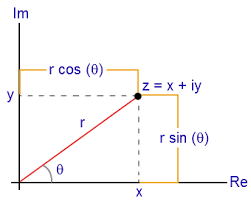
\includegraphics[width=0.5\linewidth]{Argand_plane}
	\caption{The Argand Plane.}
	\label{fig:argand}
\end{figure}
}

\begin{lemma}
	The Triangle Inequality is:
	$$\norm{z_1 + z_2} \leq \norm{z_1} + \norm{z_2}$$
	We can prove this using the argand representation. 
\end{lemma}

Properties of complex numbers:

\begin{itemize}
	\item Commutative
	\item Associative
	\item Distributive
	\item $z_1 -z_2 = z_1 + (-z_2)$.
	\item $z^n = r^n(\cos(n\theta) + i \sin(n\theta)$
	\item Complex Cojugate: $z^* = \bar{z} = x-iy = r(\cos\theta - i \sin\theta)$
	\item $z z^* = \norm{z}^2$
	\item Division 
\end{itemize}

\Def{Roots of Unity}{Given a complex number $z_0$ characterized by $r_0, \theta_0$, can we find a $z$ such that $z^n = z_0$? Well, clearly:
$$r^n = r_0$$
$$\cos(n\theta) + i \sin(n\theta) = \cos(\theta_0) + i \sin(n\theta_0)$$

This, $\norm{z} = r_0^{1/n}$, and $n\theta = \theta_0 + 2k\pi,\ k = 0, \pm 1, \pm 2...)$ There are only $n$ different solutions, meaning there are only $n$ roots. If we let $z_0 = 0$, we can find the roots of unity:

$$\text{roots of unity} = z = \cos(\frac{2k\pi}{n}) + i \sin(\frac{2k\pi}{n})$$
If we let $\omega = \cos(\frac{2\pi}{n}) + i \sin(\frac{2\pi}{n})$, then $\sum_{k=0}^{n-1} \omega^k = 0$

TODO: rebecca, this seems a bit wrong. See \href{https://en.wikipedia.org/wiki/Root_of_unity}{https://en.wikipedia.org/wiki/Root\_of\_unity} for a better explanation.

Essentially, geometrically, this means that the powers of $\omega$ sum to zero, as in Figure \ref{fig:3rdrootsofunity}.

\begin{figure}[H]
	\centering
	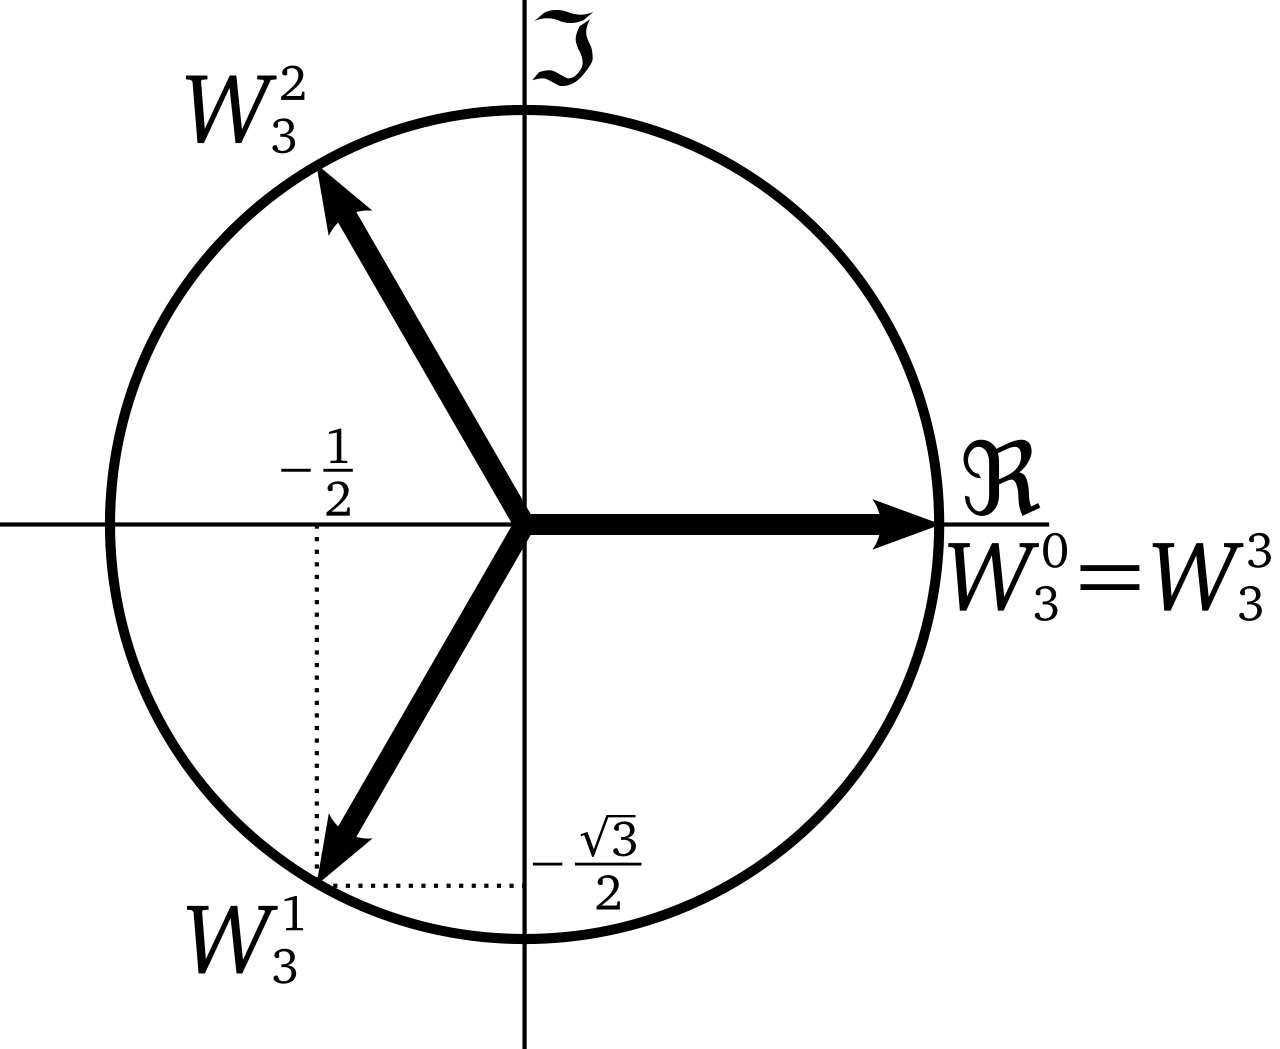
\includegraphics[width=0.5\linewidth]{3rd_roots_of_unity}
	\caption{The third roots of unity sum to one - as do nth roots of unity. \textit{Wikipedia.}}
	\label{fig:3rdrootsofunity}
\end{figure}

}

The complex numbers lack the notion of order, in the way the real numbers have order. In particular, the notion of $\infty$ is very different. For real numbers, we have $\pm \infty$, which serves as an upper and lower bound on $\R$. For complex numbers, we define a \textit{point at infinity}. The point at infinity is the limit of what happens as $r$ goes to infinity for $z=r e^{i\theta}$, While it may seem like this goes to a different point for different $\theta$, the point at infinity is in fact the same.

One way to imagine this is to consider the \textit{stereographic projection} (Figure \ref{fig:stereographic}):
\begin{figure}[H]
	\centering
	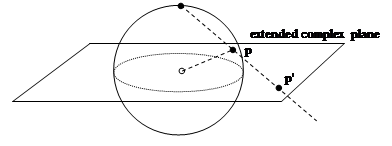
\includegraphics[width=0.5\linewidth]{stereographic_projection}
	\caption{The stereographic projection. We can see that as the point picked to move away from the point at infinity (the north pole), becomes horizontal. The intersection point on the sphere will gradually move closer to the point at the north pole, hence the north pole is the point at infinity. \textit{MathPages}.}
	\label{fig:stereographic}
\end{figure}


\subsection{Real and imaginary pairs of Z}

\begin{align}
	f(z) = u(x,y)+iv(x,y)
\end{align}

The continuity of $f(z)$ is continuous at $z = x_0 + iy_0$ $\iff u(x,y)$ and $v(x,y)$ are continuous at $x_0, y_0$ 

\subsection{Differentiation of complex functions}

\Def{Differentiable}{A function $f$ is differentiable at point $z$ if 
\begin{itemize}
	\item $\lim_{h\to0} \frac{f(z+h) - f(z)}{h} = f'(z)$ exists
\end{itemize}

\textbf{Note:} $h \in \C$ and can approach zero along any path. 
}


\begin{ex}
$f(z) = z^2$ is everywhere differentiable. 
\end{ex}

\begin{ex}
	$f(z) = |z|$ is continuous, but not differentiable at $z = 0$. 
	
	If we look at the definition:
	
	$\lim_{h\to0} \frac{f(z+h) - f(z)}{h} = \lim \frac{|h|}{h}$
	
	but $|h|$ approaches 0 so the limit does not exist.
\end{ex}



\begin{theorem}[Differential of a Complex function]
\begin{enumerate}
	\item If $f(z) = z^m$, m is integer, then $f'(z) = mz^{m-1}$
\end{enumerate}
If $f(z)$ and $g(z)$ are differentiable, then:
\begin{enumerate}
	\item$(f+g)' = f'+g'$
	\item$(fg)' = f'g + fg'$
	\item$(f/g)' = \frac{f'g-fg'}{g^2},\ g \neq 0 $
\end{enumerate}


Suppose g is differentiable at z and f is differentiable at g(z). If F(z)=f(g(z)), then:

$$ F'(z) = f'(g(z))g'(z)$$

Suppose that $h \to 0$ along the real axis. Then:

\begin{align}
\frac{f(z+h) - f(z)}{h} & = \frac{u(x+h, y) + iv(x+h,y) - u(x,y) - iv(x,y)}{h}\\
& = \frac{u(x+h, y) - u(x,y) }{h} + i \frac{v(x+h,y) v(x,y)}{h}
\end{align}

If f is differentiable at z = x+iy, both limits (as $h \to 0$) must exist and:

$$f'(z) = \frac{\partial u}{\partial x} + i  \frac{\partial v}{\partial x}$$

Next, suppose that h = ik, $k \in \R$.

\begin{align}
\frac{f(z+h) - f(z)}{h} & = \frac{u(x, y+k) + iv(x,y+k) - u(x,y) - iv(x,y)}{ik}\\
& = \frac{u(x, y+k) - u(x,y) }{ik} + i \frac{v(x,y+k) v(x,y)}{ik}
\end{align}

Since f is differentiable, both limits as $k \to 0$ must exist. We can conclude that:

$$f'(z) = \frac{\partial v}{\partial y} - i  \frac{\partial u}{\partial y}$$

We conclude that:


$$\boxed{f'(z) = \frac{\partial u}{\partial x} + i  \frac{\partial v}{\partial x} = \frac{\partial v}{\partial y} - i  \frac{\partial u}{\partial y}}$$


We can additionally conclude the \textbf{Cauchy-Riemann Conditions}:

$$\frac{\partial u}{\partial x} = \frac{\partial v}{\partial y},\ \frac{\partial v}{\partial x} = -\frac{\partial u}{\partial y}$$

\end{theorem}

\Def{Cauchy-Riemann Equations}{For a function $f(z) = u(x,y)+iv(x,y)$:
	$$\frac{\partial u}{\partial x} = \frac{\partial v}{\partial y},\ \frac{\partial v}{\partial x} = -\frac{\partial u}{\partial y}$$
	
	These furnish a necessary condition for differentiability at a point.
	
	\begin{remark}
		The Cauchy-Riemann equations are necessary, but \textbf{not} sufficient for differentiability at a point.
\end{remark}}

\begin{ex} Consider the complex conjugate function:
	$$f(z) = z^* = \bar{z} = x-iy$$
	
	We would like to determine if $f$ is differentiable. If it is, it must satisfy Cauchy-Riemann equations.
	
	$$\frac{\partial u}{\partial x} = 1,\ \frac{\partial v}{\partial y} = -1$$
	
	Already, we see that $\frac{\partial u}{\partial x} \neq \frac{\partial v}{\partial y}$. So $f(z)$ is not differentiable for any value of z.
\end{ex}

\begin{remark}
The Cauchy-Riemann equations can also be written as:

$$f'(z) = \frac{\partial f}{\partial x} = -i \frac{\partial f}{\partial y}$$

\end{remark}


\begin{theorem}
	Let $f=u+iv$ be differentiable with complex partials at $z=re^{i\theta}$. Then:
	$$\pdv{u}{r} = \frac{1}{r} \pdv{v}{\theta},\ \pdv{v}{r} = -\frac{1}{r} \pdv{u}{\theta}$$
\end{theorem}


\Def{Analyticity}{A function is \textbf{analytic (holomorphic) }at a point if it is differentiable everywhere in some neighborhood of the point. If the function is analytic for all values of $z \in \C$, then it is \textbf{entire}. 
	
Note: Being differentiable in a neighborhood (analytic) is a stronger requirement than just differentiable. 

\textbf{Remark:} If a function is analytic at a point, it is differentiable for all orders at that point.
}


\begin{ex} Let 
$f(z) = |z|^2 = z \bar{z}$. This function is differentiable only at $z=0$, but it is nowhere analytic. 
\end{ex}

\begin{theorem}Let $f(z) = u(x,y)+iv(x,y)$  be defined in a domain D. Let $u(x,y)$ and $v(x,y)$ have continuous partials that satisfy Cauchy-Riemann equations for all points in D. Then, we can show that $f(z)$ is analytic in D. Thus, Cauchy-Riemann applied to the neighborhood is sufficient to show analyticity.
\end{theorem}

\begin{ex}
$f(z)=e^z = e^z=e^x(\cos y + i \sin y)$


Therefore, $e^z$ is an entire function. 

$$f'(z) = e^z$$
\end{ex}

Note: if $f$ is analytic of non-zero at a point z, then a branch may be chosen for which $\log (f(z))$ is also analytic in the neighborhood of z and $\dv{}{z} log(f(z)) = \frac{f'(z)}{f(z)}$


\subsection{Branch points and Branch Cuts}
Explaining the epsilon method: \url{https://math.stackexchange.com/questions/2150639/branch-point-of-logz}
The easy way to do branch points is to remember that $log(z)$ and $z^p$ where p is non integer both have branch points at $0, \infty$. So simply find when $z = 0, \infty$ for those functions to get the branch points. Then a branch cut must connect all branch points, but does not have to go in any particular way. For $log(z)$, the negative real line is often the branch cut that is picked.


Branch points are points where the function is non-analytic. 

\subsection{Harmonic functions}
Later, we will see that analytic functions have derivatives of all orders. Recall:
$$f'(z) = \frac{\partial f}{\partial x} = -i \frac{\partial f}{\partial y}$$

We can take the derivative:

$$f''(z) = \frac{\partial f}{\partial x} = -i \frac{\partial f}{\partial y}$$
And so:
$$\pdv{^2f}{x^2} + \pdv{^2f}{y^2} = 0$$

Since $f(z) = u(x,y) + i v(x,y)$, 

$$\pdv{^2u}{x^2} + \pdv{^2u}{y^2} = 0 \pdv{^2v}{x^2} + \pdv{^2v}{y^2} = 0$$

\Def{Harmonic Function}{ A continuous, real valued function u(x,y) defined on domain D is called \textbf{harmonic} if it has continuous first and second derivatives, satisfying Laplace's equation:
$$\pdv{^2u}{x^2} + \pdv{^2u}{y^2} = 0$$ 

Note: The real and imaginary parts of an analytic functions are harmonic functions.}

\Def{Harmonic Conjugate}{If $f(z) = u + iv$ is analytic, $v$ is called the harmonic conjugate of $u$, and vice versa.}

\begin{remark}
Laplace's equation furnishes a \textbf{necessary} condition for a function to be real and imaginary parts of an analytic function.
\end{remark}

\begin{ex}
$u(x,y) = x^2+y$

This cannot be the real part of any analytic function, since the Laplace equations are not satisfied. $$\pdv{^2u}{x^2} + \pdv{^2u}{y^2} \neq 0 $$.
\end{ex}

\Section{Sequences}
\Def{Sequence}{ A sequence $\{z_n\}$ of complex numbers is an assignment of a complex number $z_n$ to each positive integer $n$.}

\Def{Convergent sequence}{A sequence $\{z_n\}$ is said to have a limit $z_0$ or converge to $z_0$ which we write as 

$$\lim_{n\to\infty} z_n = z_0$$

if for every $\epsilon > 0, \exists\ M \in  \mathbb{Z}$, such that:

$$|z_n - z_0| < \epsilon,\ \forall n > M$$

This means for sufficiently large values of $n$, $z_n$ is arbitrarily close to $z_0$.

\begin{figure}[H]
	\centering
	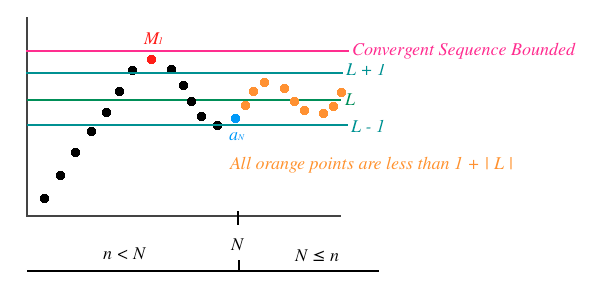
\includegraphics[width=0.7\linewidth]{convseq}
	\caption{A convergent sequence example. }
	\label{fig:convseq}
\end{figure}

Alternative definition: Every neighborhood of $z_0$ contains all but a finite number of $z_n$'s.
}

\begin{ex}
$\{\frac{1}{m}\}$ converges to 0. However, $\{(-1)^{m}\}$ does not converge. 
\end{ex}

\begin{theorem}
Let $z_m = x_m + i y_m$ be a sequence of complex numbers $\{z_m\}$. Then, this converges to $z_0 = x_0 + i y_0$ if and only if the real sequences $\{x_m\}, \{y_m\}$ converge to $x_0, y_0$ respectively.

\textbf{Remark}: The properties of complex sequences can be derived from corresponding properties of real sequences. For example, the uniqueness of the limit (can only converge to one value).
\end{theorem}

\begin{theorem}
A convergent sequence is bounded. 

\textbf{Proof:}

If $\lim_{m\to\infty}z_m = z_0$, then there must be a $z_m \in N(z_0,1)$ , where $N$ means neighborhood, for $m>N$, let $M = \max\{|z_1|, .., |z_N|\}$, then
$$|z_m| < M + |z_0| + 1, \forall m$$

Note that the converse is not true. Counterexample:

$\{1,2,1,2,1,2\}$ is bounded but does not converge. 
\end{theorem}
\Def{Subsequence}{A subsequence of $\{z_m\}$ is a sequence $\{z_{m_k}\}$ whose terms are selected from the terms in an original sequence and arranged in the same order. Subsequences may converge even if sequences do not.}
\begin{ex}
Given a sequence $z_m = (-1)^{m}$, a subsequence could be $z_{m_k} = z_{2k}$, or the even terms, which results in $\{1,1,..1\}$ which converges to 1. The subsequence $z_{m_k} = z_{2k+1}$ converges to -1.
\end{ex}

\begin{theorem}
If a sequence $\{z_m\}$ converges to $z_0$, then every subsequence also converges to $z_0$. 
\end{theorem}

\begin{theorem}
Every bounded sequence of complex numbers contains at least one convergent subsequence. 

\textbf{Proof:} Exercise. 
\end{theorem}

\Def{Cauchy Sequence}{A sequence is Cauchy sequence if in the limit, the difference between the terms becomes arbitrarily small (each value becomes arbitrarily close to each other), which lets us not define the actual limit. 

Formally, a sequence $\{z_m\}$ of complex numbers is a Cauchy sequence if for every $\epsilon>0$, $\exists N \in \mathbb{Z}$ such that $|z_m - z_M| < \epsilon,\ \forall m, M>N$.}

\begin{theorem}
A sequence $\{z_m\}$ converges if and only if $\{z_m\}$ is a Cauchy sequence. 

Note: The two notions of convergence and Cauchy convergence are equivalent. Cauchy convergence is the most general test of convergence. It works even if the limit $z_0$ is not known.
\end{theorem}

\Section{Series}
\Def{Series}{Given a complex sequence $\{a_m\}$, we associate a new sequence defined by $s_m = \sum_{k=1}^{n}a_k$. Then, we say that $\sum_{k=1}^{\infty}a_k$ is a series. The series is said to converge or diverge according to whether the sequence $\{s_m\}$ converges or diverges. We call $\{s_m\}$ the \textbf{partial sum} of the series, and $a_k$ the kth term.

\textbf{Note:} Every theorem about sequences can be rephrased to be a theorem about series, since series are sequences, and vice versa
}
\begin{theorem}
Let $\{a_m\}$ be a sequence of complex numbers, with $a_m = \alpha_m+ i \beta_m$ where $\{\alpha_m\}, \{\beta_m\}$ are sequences of real numbers. Then, by the earlier result, the complex series $\sum_{k=1}^{\infty}a_k$ converges if and only if $\sum_{k=1}^{\infty}\alpha_k$ and $\sum_{k=1}^{\infty}\beta_k$ converge.
\end{theorem}


\Def{Cauchy Criterion.}{Let $s_m = \sum_{k=1}^{m}a_k$. The series $\sum_{k=1}^{\infty}a_k$ converges if and only if for every $\epsilon>0$, there exists $N \in \mathbb{Z}$ for $m, M>N$:

$$|s_M - s_m| = \left|\sum_{k=m+1}^{M}a_k\right| < \epsilon$$

Alternatively, letting $M = m+p$:

$$|s_{m+p} - s_m| = \left|\sum_{k=m+1}^{m+p}a_k\right| < \epsilon, \forall p = 1,2,3,..$$

This is the most general test for convergence of a series. 

Note: Familiar properties of a series are immediate consequences of the Cauchy criterion.

Note: $a_k \to 0$ to converge. (set $p=1$).
 }

\Def{Absolutely Convergence}{A series $\sum_{m=1}^{\infty}a_m$ is said to be absolutely convergent if $\sum_{m=1}^{\infty}|a_m|$ converges. 

\textbf{Note:} Applying the triangle inequality:

$$\left|\sum_{k=m+1}^{m+p}a_k\right| \leq \sum_{k=m+1}^{m+p}\left|a_k\right|$$

Applying this with the Cauchy criterion, we can deduce that absolute convergence of a series ensures its convergence. 

\textbf{Note:} If $|a_m| \leq |b_m|$, for every $m$, the convergence of $\sum_{m=1}^{\infty} |b_m|$ implies convergence of $\sum_{m=1}^{\infty} |a_m|$ .
}

\begin{theorem}
Suppose $a_m>0\ \forall m$ and that $\sum_{m=1}^{\infty} a_m$ diverges. If $s_m = \sum_{k=1}^m a_k$, then:
\begin{enumerate}
	\item $\sum_{m=1}^{\infty} \frac{a_m}{s_m}$ also diverges.
	\item $\sum_{m=1}^{\infty} \frac{a_m}{s_m^2}$ also converges. This is shown by Cauchy. 
\end{enumerate}
\end{theorem}

\begin{corollary}
The series 	$\sum_{m=1}^{\infty} \frac{1}{m}$ also diverges. But $\sum_{m=1}^{\infty} \frac{1}{m^2}$ converges.
\end{corollary}

\begin{theorem}[Geometric series]
Consider $s_m = \sum_{k=1}^m r^{k-1} = \frac{1-r^m}{1-r}$. This is a geometric series.  

\textbf{Proof:}

\begin{align}
(1-r)\sum_{k=1}^m r^{k-1} &= \sum_{k=1}^m r^{k-1} - r^k \\ 	
& = 1-r^m
\end{align}

Hence a series $\sum_{m=1}^\infty a_m$ converges absolutely if ther eexists a constant $r \in [0,1)$ and a real number M such that $|a_m| < M r^m,\ m>M$
\end{theorem}

\subsection{Limits of series and sequences}
\Def{Limit Superior }{Let $\{a_m\}$ be the real bounded sequence and let A be the set of subsequence limits of $\{a_m\}$. We define the limit $\sup$ of $\{a_m\}$ as the least upper bound of A:

$$\lim\sup_{m \to \infty }a_m = L.U.B.\{A\}$$

\textbf{Note:} If $\{a_m\}$ is unbounded above, then:

$$\lim\sup_{m \to \infty }a_m = + \infty $$


Note: If all but a finite number of $a_m$ are less than any pre-assigned real number, we say that :

$$\lim\sup_{m \to \infty } a_m = - \infty $$
}



\Def{Limit Inferior}{Let $\{a_m\}$ be the real bounded sequence and let A be the set of subsequence limits of $\{a_m\}$. We define the limit $\inf$ of $\{a_m\}$ as the greatest lower bound of A:
	
	$$\lim\inf_{m \to \infty }a_m = G.LB.\{A\}$$
}

Note: in the extended reals $(\R \cup \pm \infty)$, the limit superior and limit inferior of a real sequence always exists. This allows us to state and prove results without worrying about the existence of limits.

\begin{theorem}
Let $\{a_m\}$ and $\{b_m\}$ be real valued sequences. Then, 
\begin{enumerate}
	\item $\lim \sup_{m \to \infty }(a_n + b+m) \leq \lim\sup a_m + \lim\sup b_m$
	\item $\lim \inf_{m \to \infty }(a_n + b+m) \leq \lim\inf a_m + \lim\inf b_m$
\end{enumerate}
\end{theorem}

\begin{remark}
\textbf{On the difference between limsup and sup}
\url{https://math.stackexchange.com/questions/1734087/difference-between-limsup-and-sup}

\end{remark}

\begin{theorem}[Root Test]
Let $\{a_m\}$ be a complex sequence and suppose that:
$$\lim\sup_{m \to \infty } |a_m|^{1/m} = L$$

Then the series $\sum_{m=1}^\infty a_m$ converges absolutely if $L<1$ and diverges if $L>1$. 

\textbf{Proof:}

Case 1: \\ 
If $L<1$, choose $r$ such that $L<r<1$. For all but a finite number of m, we have that:

\begin{align}
|a_m|^{1/m} & < r \\ 
|a_m|&  < r^m  
\end{align}

This is true since by the definition of $L$, this must be true. 

The convergence of $\sum_{m=1}^\infty a_m$ now follows from convergence of $\sum_{m=1}^\infty r^m$, $r<1$.

Case 2:\\
If $L>1$, then $|a_m|^{1/m} >1$ for infinitely many values of $m$. But then $|a_m|>1$ infinitely often. Then $a_m \not \to 0$ and the series diverges. 

Case 3: \\ 
If $L=1$, the root test does not give any information.

\textbf{Ex:} $\sum \frac{1}{m}$ diverges, but $\sum \frac{1}{m^2}$ converges.

 However, $\lim\sup_{m \to \infty }|\frac{1}{m}|^{1/m} = 1$. Similarly, $\lim\sup_{m \to \infty }|\frac{1}{m^2}| = 1$

\end{theorem}

\subsection{Convergence}
\Def{Pointwise Convergence}{A sequence of functions $\{f_m(z)\}$ converges pointwise to a function $f$ on a set $E$ $(f_m \to f)$, if to each $z_0 \in E$, and $\epsilon>0$, there corresponds  and integer $N = N(\epsilon, z_0)$ for which $|f_m(z_0) - f(z_0)|<\epsilon$ whenever $m>N$.

Pointwise convergence implies $\lim_{m\to\infty} f_m(z_0) = f(z_0)$


Note: the integer $N$ may, in general, vary with $z_0 \in E$. If one integer can be found that works for all $z_0 \in E$, then we have a special (stronger) type of convergence: \textbf{uniform convergence.}
}

\Def{Uniform Convergence}{A sequence of functions $\{f_m\}$ converges uniformly to $f$ on set $E$ $(f_m \Rightarrow f)$, If for each $\epsilon>0$ there corresponds an integer $N = N(\epsilon)$ such that for all $z \in E$, $|f_m(z_0) - f(z_0)| < \epsilon$ whenever $m>N$.}

\begin{ex}
Consider $f_m(z) = \frac{1}{mz}$ . This converges pointwise but not uniformly to $f(z)=0$ in the set $0<|z|<1$. This is because uniform convergence would require existence of $N$ such that $\left|\frac{1}{mz}\right| < \epsilon < 1$ valid for all $z$ in the set. You can see this is not true in the case $z = \frac{1}{n}$. $f(\frac{1}{n})$ would be greater than $1$, so yeah. 
\end{ex}

The importance of uniform convergence is that it allows for the interchange of many limiting operations.  which, in turn, compels the limit to retain many properties of sequences.

\begin{theorem}
Suppose $\{f_m\}$ converges uniformly to $f$ on $E$. If each $f_m$ is continuous at point $z_0 \in E$, the limit of the function $f$ is also continuous at $z_0$:

$$\lim_{z \to z_0} \lim_{m \to \infty }f_m(z) = \lim_{m \to \infty }\lim_{z \to z_0}f_m(z)$$


The provides a necessary condition for uniform convergence.
\end{theorem}

\begin{ex}
$f_m = \frac{1}{1_mz}$. This converges pointwise to 

\begin{align}
f = \begin{cases}
0 & if\ z\neq 0 \\ 1 & if\ z = 0 \\ 
\end{cases}
\end{align}

Since $f$ is not continuous, the convergence cannot be uniform in any region containing the point $z=0$. 
\end{ex}

Note, this generalizes cauchy convergence. 



\subsection{Series of Complex Functions}
Given a sequence of functions $\{f_m\}$ defined on the set $E$, we associate a new sequence $\{s_m(z)\}$ defined by 
$$s_m(z) = \sum_{k=1}^m f_m(z)$$

For values for which  $\lim_{m \to \infty }s_m(z)$ exists, we say the series converges. 

\begin{align}
f(z) &= \lim_{m \to \infty } \sum_{k=1}^m f_k(z) \\ 
& = \sum_{k=1}^\infty f_k(z)
\end{align}

Note, this is different than before. Now $f(z)$ is the limit of the sum, not just the limit.

If $\{s_m(z)\}$ converges uniformly on $E$, then the series $\sum_{k=1}^\infty f_k(z)$ is said to be \textbf{uniform} on $E$. Similarly, if $\sum_{k=1}^\infty f_k(z)$ is uniformly convergent on $E$, then
$\sum\left|f_m(z)\right|$ converges. 

\begin{theorem}
The series $\sum_{m=1}^\infty f_m(z)$ converges uniformly on a set $E$ if and only if to each $\epsilon$, there corresponds an integer $N = N(\epsilon)$, such that for all $z \in E$, 
\begin{align}
\left|\sum_{k=m+1}^{m+p}f_k(z) \right| < \epsilon,\ m>N,\ p = 1,2,3..
\end{align}


By the triangle inequality, this also implies absolute convergence. 
\end{theorem}

\begin{theorem}[Weirstrass M-test]
Let $M_m$ be a sequence of real numbers. Suppose that $|f_m(z)| < M_m, \forall z \in E, m\in \mathbb{Z}^+$.  If $\sum_{m=1}^\infty M_m$ converges, then $\sum_{m=1}^\infty f_m(z)$ converges uniformly and absolutely on $E$. 
\end{theorem}
\begin{ex}
The series $\sum_{m=1}^\infty z^m $ converges absolutely for $|z|<1$. It converges uniformly for $|z|\leq r < 1$. 
\end{ex}

Note: $\sum_{m=1}^\infty |z^m| = \sum_{m=1}^\infty |z|^m = \frac{|z|}{1-|z|},\ |z|<1$. This proves absolute convergence for $|z|<1$. 


Let $M_m = r^m$. Then $|z^m| \leq r^m$ for $|z| \leq r < 1$. But $\sum_{m=1}^\infty r^m$ converges for $r<1$. So: $\sum_{m=1}^\infty z_m$ converges uniformly for $|z| \leq r < 1$. This follows from the Weirstrass M-test. 

\Section{Power Series}
\Def{Power Series}{Let $f_m(z) = a_m(z-b)^m$ where $a_m, b$ are complex. $\sum_{m=1}^\infty f_m(z) = \sum_{m=0}^\infty a_m(z-b)^m$ is a called a power series in $z-b$. WLOG, set $b=0$. }

\begin{theorem}
Suppose a power series $\sum_{m=0}^\infty a_m z^m$ converges at point $z=z_0$. Then $\sum_{m=0}^\infty |a_m| |z|^m$ converges for $|z|<|z_0|$. 

Basically, if it converges at $z_0$, then it converges in a disc centered at $b$ with radius $z_0-b$. 

\textbf{Proof:} Since $\sum_{m=0}^\infty a_m z_0^m$ converges, we have that $\lim_{m \to \infty }a_m z_0^m = 0$. Hence there is a constant $M$ such that $\left|a_mz_0^m\right|<M,\ \forall m$. Also:

$$|a_m| |z|^m =\left| a_m z_0^m \left(\frac{z}{z_0}\right)^m \right| < M \left|\frac{z}{z_0}\right|^m$$
For $|z|<|z_0|$, the geometric series $\sum_{m=0}^\infty \left|\frac{z}{z_0}\right|^m$ converges. Thus:

$$\sum_{m=0}^\infty |a_m| |z|^m \leq \sum_{m=0}^\infty \left|\frac{z}{z_0}\right|^m = \frac{M}{1-\left|\frac{z}{z_0}\right|},\ |z|<|z_0|$$
\end{theorem}

\begin{corollary}
If $\sum_{m=0}^\infty a_m z^m$ diverges at $z = z_0$, then $\sum_{m=0}^\infty a_m z^m$ diverges for $|z| > |z_0|$. 
\end{corollary}

\begin{corollary}
Of $\sum_{m=0}^\infty a_m z^m$ converges for all real values of z, then the series also converges for all complex values.	\end{corollary}
\begin{theorem}
For every power series $\sum_{m=0}^\infty a_m z^m$, there correspondes a number $R \in [0, \infty]$ for which it satisfies:
\begin{enumerate}
	\item It converges absolutely in $|z| < R$
	\item It converges uniformly in $|z|\leq R_0 < R$ 
	\item It diverges for $|z|>R$.
\end{enumerate}

\textbf{Proof:} Let $s = \{r\ s.t.\ \sum_{m=0}^\infty a_m z^m\text{ converges for } |z|<r\}$. Then $R = \begin{cases}
L.U.B. s \text{ if } s \text{is bounded} \\ 
\infty \ otherwise
\end{cases}$

Note: $R$ is the radius of convergence of a power series. It converges inside, diverges outside the circle $|z| = R$. On the other hand, it may converge at all some, or none of the points on the circle $|z|=R$. 

\end{theorem}

\begin{theorem}
The power series $\sum_{m=0}^\infty a_m z^m$ has a radius of convergence $R = \frac{1}{A}$, where $A =\lim\sup_{m \to \infty } |a_m|^{1/m}$. If $A = \infty$, $R = 0$. Likewise, if $A=0$, $R = \infty$. 

\textbf{Proof:}
For any point $z_0$, $\lim\sup_{n \to \infty } |a_nz_0^n|^{1/n} = \left(\lim\sup_{n \to \infty }|a_n|^{1/n}\right)$. According to the root test, the series $\sum_{m=0}^\infty a_m z^m$ converges absolutely when $|z_0|A < 1$ 

\textbf{Note:} $f(z) = \sum_{m=0}^\infty a_m z^m$ is continuous at $z = z_0$ with $|z_0|<R$. what about differentiation?
\end{theorem}


\begin{theorem}
If a function $f(z)$ is the pointwise limit of a power series $\sum_{m=0}^\infty a_m z^m$ in $|z|<R$,
\end{theorem}
See other notes of 9/23-9/25 for a description of what happened here.

\Section{Contours}

Note: If f is analytic in domain including $C$, we can find $F$ such that $F'=f$

\begin{theorem}[Cauchy's Theorem]
If $f(z)$ is analytic in a Domain D and C is a closed contour lying on D, then $$\int_{C} f(z) dz = 0$$

\textbf{Note:} the argument use to generalize the weaker version of Cauchy for multiply connected regions can be repeated for the stronger version

\textbf{Note:} this takes the work of parameterizing ugly contours, as will be seen in the next example.
\end{theorem}

\begin{ex}
Evaluate $\int_C \frac{1}{z-z_0}dz$ for some arbitrary ugly contour
Define a nice contour $C_1 : |z-z_0| = \epsilon$ which is a circle completely inside $C$, such taht it does not divide the interior region.

Now, $f(z) = \frac{1}{z-z_0}$ is analytic in a multiply connected region between $C$ and $C_1$. Hence
$$\int_{C+C_1}f(z)dz = 0$$

Therefore, $\int_C \frac{1}{z-z_0}dz = -\int_{C_1} \frac{1}{z-z_0}dz$. 

Since $C_1 : z(t) = z_0 + \epsilon e^{it},\ t \in [0, 2\pi]$. Thus, 

$$\int_C \frac{1}{z-z_0}dz = \int_{0}^{2\pi}\frac{z'(t)}{z(t)-z_0} dt = \int_{0}^{2\pi} \frac{i\epsilon e^{it}}{\epsilon e^{it}} dt = 2\pi i$$
\end{ex}

\Def{Laplace Transform}{$$F(s) = \int_{0}^{\infty} e^{-st} f(t) dt$$

The inversion of the Laplace transform involves an integral on the complex plane of a vertical contour to the right of all singularities. 

$$f(t) = \frac{1}{2\pi}\int_{\gamma - i \infty}^{\gamma + i \infty} F(s) e^{st}ds $$

There is a trick where you can close the contour to the right if there are no singularities to the right of the contour. Then, this causes $f(t)$ to have a zero contribution from the point at infinity. This only happens if $t<0$. This is usually true as $f(t)$ is usually zero before $t=0$.}


\begin{theorem}[Cauchy Integral Formula]
	
Let $f(z)$ be analytic in a simply connected domain containing the simple closed contour C. If $z_0 \in C$, then 

$$f(z_0) = \frac{1}{2\pi i}\int_{C} \frac{f(z)}{z-z_0}dz$$

\begin{figure}[H]
	\centering
	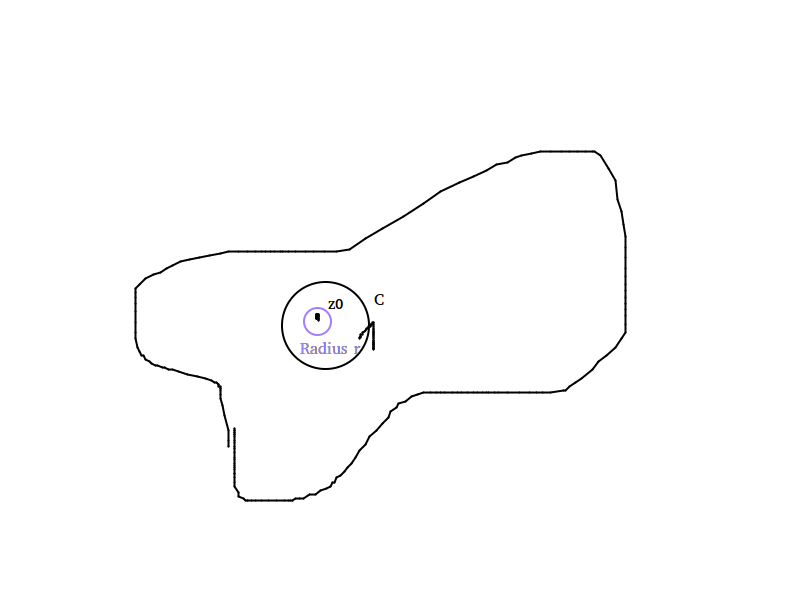
\includegraphics[width=0.7\linewidth]{intform}
	\caption{Contour for Cauchy integral Form on some domain.}
	\label{fig:intform}
\end{figure}

Note: $f(z)=1$ is the previous example.

Roughly speaking, if $z_0$ in the integral, then $\frac{f(z)}{z-z_0}dz = 2\pi i f(z_0)$. If it is outside $C$, the value of the integral is zero. 

\textbf{Proof:}

Given $\epsilon>0$, construct a circle $C_1: |z-z_0|=r$. And small enough $r$ such that $|f(z) - f(z_0)|<\epsilon$ for all $z$ on $C_1$. By Cauchy's theorem:

\begin{align}
\int_C \frac{f(z)}{z-z_0}dz &= \int_{C_1} \frac{f(z)}{z-z_0}dz\\ 
& = \int_{C_1} \frac{f(z_0)}{z-z_0}dz +  \int_{C_1} \frac{f(z) - f(z_0)}{z-z_0}dz\\
 & = 2 \pi i f(z_0) +  \int_{C_1} \frac{f(z) - f(z_0)}{z-z_0}dz
\end{align}

However:

\begin{align}
\left|\int_{C_1} \frac{f(z) - f(z_0)}{z-z_0}dz \right| &\leq \int_{C_1} \frac{|f(z) - f(z_0)|}{|z-z_0|}dz \\
&< \int_{0}^{2\pi} \frac{\epsilon}{r} |dz| = \epsilon 2 \pi 
\end{align}

This goes to zero as $\epsilon \to 0$. Thus, $\int_C \frac{f(z)}{z-z_0}dz = 2 \pi i f(z_0)$

\textbf{Note:} The theorem expresses the value of $f(z)$ at any point in $C$ in terms of values of $f$ on $C$ (no real valued analog to this result).
\end{theorem}

\begin{theorem}[Cauchy Integral Formula for Derivative]
Let $f(z)$ be analytic on a simply connected domain containing a closed simple contour $C$. Then, $f(z)$ has derivatives of all orders at each point $z_0 \in C$. Moreover, the $nth$ derivative at that point is:
$$f^{(n)}(z_0) = \frac{n!}{2\pi i } \int_C \frac{f(z)}{(z-z_0)^{n+1}}dz$$

\textbf{Proof:}
Use the previous result with the definition of the derivative. Assume that $h$ is small enough such that $z_0+h$ is inside $C$. Then:

\begin{align}
\frac{f(z_0+h) - f(z_0)}{h}& = \frac{1}{2\pi i h } \left(\int_C \frac{f(z+h)}{z-z_0-h} dz - \int_C \frac{f(z)}{z-z_0}dz \right)\\
&= \frac{1}{2\pi i } \int_C \frac{f(z)}{(z-z_0)(z-z_0-h)} dz
\end{align}

As $h \to 0$, we see $f'(z_0) = \frac{1}{2\pi i h } \int_C \frac{f(z)}{(z-z_0)^2} dz$. However, it is hard to take the limit of an integral so this is hard, so we have to argue this.
\end{theorem}

\textbf{Note:} We know by hypothesis that $f(z)$ was differentiable at all $z_0$ inside $C$. The theorem demonstrates the existence of all derivatives of $f(z)$. 

\textbf{Note:} If $f$ is analytic at $z_0$, it is differentiable to all orders there. 

\textbf{Note:} The Cauchy-integral formula is also valid for multiply connected domains.

\begin{ex}
\begin{figure}[H]
	\centering
	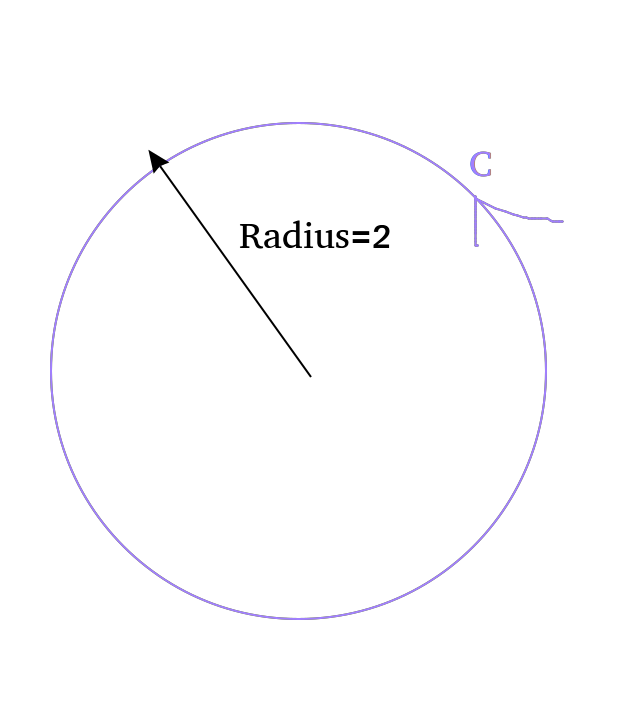
\includegraphics[width=0.4\linewidth]{example12}
	\caption{}
	\label{fig:example12}
\end{figure}


$$\int_{|z|=2}\frac{z-3\cos z}{(z-\pi/2)^2}dz$$

Let $f(z) = z-3\cos z$. Then $f'(z) = 1+3 \sin z$. By the Cauchy integral Formula, 

$$\int_{C} \frac{f(z)}{(z-z_0)^2} dz = 2\pi i f'(\pi/2) = 8\pi i $$
\begin{quote}
	"Almost like magic, isn't it?"
\end{quote}
\end{ex}


\Def{Principal Value Integrals}{
If $z_0$ is outside contour $C$, then $\frac{1}{2\pi i}\int_{C} \frac{f(z)}{z-z_0}dz = 0$. If $z_0$ is on $C$, the integral does not exist. Instead, the integrand blows up "too strongly," much like the drink I'll be having tonight. However, we can re-interpret the integral so as to avoid the singularity, keeping in mind of course that such a reinterpretation is a matter of definition. Given $C$ and $z_0$ through $C$, and not having a corner there , we consider the modified contour $C'$ excluding $z_0$, putting $z_0$ on the inside. By semi-circle of radius $\epsilon>0$. Then:

$$\frac{1}{2\pi i}\int_{C'} \frac{f(z)}{z-z_0}dz = 0$$

As $\epsilon \to 0$, the part over the semicircle becomes 

$$\frac{1}{2\pi i}\int_{\pi}^0 \frac{f(z_0 + \epsilon e^{i\theta})}{\epsilon e^{i\theta}} i \epsilon e^{i\theta} d\theta = -\frac{f(z_0)}{2}$$

Using the previous theorems:

$$\frac{1}{2\pi i}\int_{C'} \frac{f(z)}{z-z_0}dz = PV \frac{1}{2\pi i}\int_{C} \frac{f(z)}{z-z_0}dz -\frac{f(z_0)}{2} =  0$$

And so:

$$PV \frac{1}{2\pi i}\int_{C} \frac{f(z)}{z-z_0}dz = \frac{f(z_0)}{2}$$

\textbf{Note:} This relies on putting the contour on the inside, but we could put it on the outside. Key feature, it doesn't matter! Wow. Now if $z_0$ is a corner point enclosing an \textbf{interior angle} of $\alpha$ radians, then the principal value is:

$$PV \frac{1}{2\pi i}\int_{C} \frac{f(z)}{z-z_0}dz = \frac{f(z_0)}{2}$$

\begin{figure}[H]
	\centering
	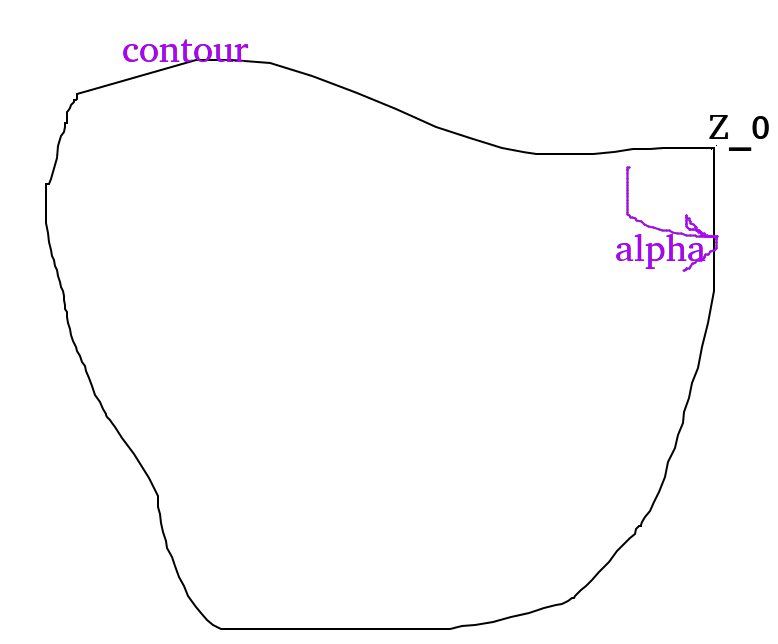
\includegraphics[width=0.5\linewidth]{angle_contour}
	\caption{}
	\label{fig:anglecontour}
\end{figure}

}

% 10/2 Notes
\begin{theorem}[Taylor's Theorem]
Let $f(z)$ be analytic in domain $D$ whose boundary is $C$. If $z_0$ is a point in $D$, then $f(z) = f(z_0) + f'(z_0)(z-z_0) + \frac{1}{2!} f''(z_0) (z-z_0)^2+...$

The series converges for $|z-z_0|<\delta$ where $\delta$ is the distance from $z_0$ to $C$. 

\textbf{Proof:}
\begin{figure}[H]
	\centering
	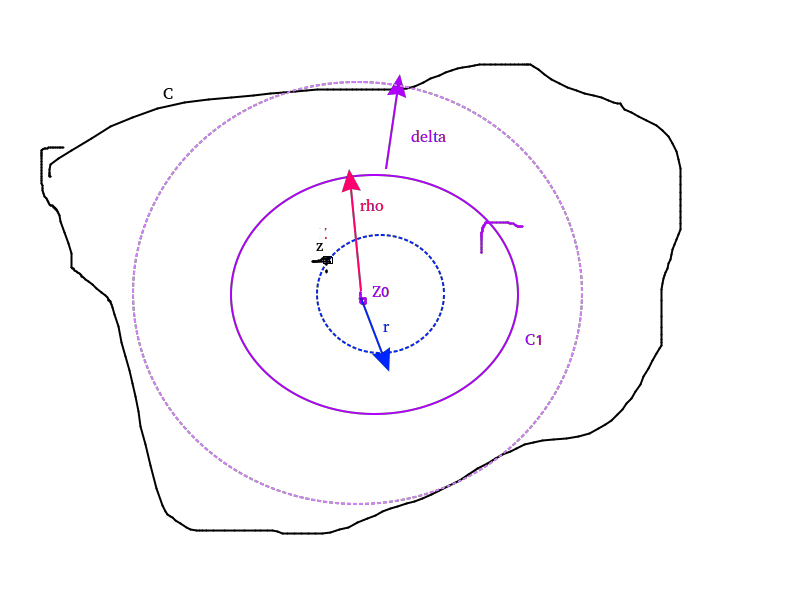
\includegraphics[width=0.5\linewidth]{disc}
	\caption{$\delta$ is the largest circle that fits inside the contour $C$}
	\label{fig:disk}
\end{figure}

Construct circle $C_1:|\zeta - z_0| = \rho$ with $\rho < \delta$. Let $z$ be any point inside $C_1$, then by C.T.M, 

$$\rho(z) = \frac{1}{2 \pi} \int_{C_1} \frac{\rho(\zeta)}{\zeta - z} d\zeta$$.

We set $|z-z_0| = r$, then $ r = |z-z_0|  < |\zeta - z_0| = \rho$. Additionally, 

\begin{align}
\frac{1}{\zeta - z} &= \frac{1}{\zeta - z_0 - (z - z_0)}\\
&= \frac{1}{\zeta - z_0} \frac{1}{1-\frac{z-z_0}{\zeta - z_0}}\\
&= \frac{1}{\zeta - z_0} \left[1 + \frac{z-z_0}{\zeta - z_0} + \left(\frac{z-z_0}{\zeta - z_0}\right)^2 + .. + \left(\frac{z-z_0}{\zeta - z_0}\right)^{n-1} + \sum_{k=m}^\infty \left(\frac{z-z_0}{\zeta - z_0}\right)^k\right] \\ 
&= \frac{1}{\zeta - z_0} \left[1 + \frac{z-z_0}{\zeta - z_0} + .. + \left(\frac{z-z_0}{\zeta - z_0}\right)^{n-1} + \frac{\left(\frac{z-z_0}{\zeta - z_0}\right)^n}{1-\frac{z-z_0}{\zeta - z_0}}\right]
\end{align}

Then 

\begin{align}
f(z) = \frac{1}{2 \pi i } \int \frac{f(\zeta)}{\zeta - z_0} d\zeta + ... + \frac{(z-z_0)^{n-1}}{2 \pi i}\int \frac{f(\zeta)}{\zeta - z_0} d\zeta + R_n
\end{align}

Where 
$$R_n = \frac{1}{2 \pi i } \int_{C_1} \left(\frac{z-z_0}{\zeta - z_0}\right)^n \frac{f(\zeta)}{\zeta - z}d\zeta$$

By Cauchy Integral Formula, we get that 

\begin{align}
f(z) = f(z_0) + f'(z_0)(z-z_0) + ... + \frac{f^{(n-1)}(z_0)}{n-1}(z-z_0)^{n-1} + R_n
\end{align}

However, we still need to show that $R_n \to 0$ as $n \to \infty$. 

For ??? assume $|f(z)| \leq M $ on $C_1$. Then,
We note that from triangle inequality $$\frac{1}{|\zeta-z|} = \frac{1}{|\zeta - z - z_0 + z_0|} \leq \frac{1}{|\zeta - z_0| - |z-z_0|} = \frac{1}{\rho - r}$$

Then we can conclude that

\begin{align}
|R_n| &\leq \frac{1}{2 \pi i } \int_{C_1} \left|\frac{z-z_0}{\zeta - z_0}\right|^n \frac{|f(\zeta)|}{|\zeta - z|}|d\zeta \\ 
&\leq \frac{M}{2 \pi i } \left(\frac{r}{\rho}\right)^n \int_{C_1} \frac{1}{|\zeta-z|}|d\zeta| \\
&\leq \frac{M}{2 \pi i } \left(\frac{r}{\rho}\right)^n \frac{1}{\rho - r} 2 \pi \rho 
\end{align}

Since $r/\rho < 1$ as $n \to \infty$, $|R_n| \to 0$

\textbf{Note:} by the M-test, the Taylor series converges uniformly on  compact subsets of disk $|z-z_0|<\delta$. 


What is this saying? We can chose any circle originating from $z_0$ with radius $R$, as long as it is less than $\delta$ which is the maximum radius to stay within the contour $C$, we will converge uniformly. (is this really true?)
\end{theorem}

We have seen before that a power series represents an analytic function inside its radius of convergence. The result in Taylor's theorem says essentially the converse. Thus, a function $f(z)$ is analytic at a point $z_0$ if and only if $f(z) = \sum_{n=0}^{\infty}a_n(z-z_0)^n$ in some disk $|z-z_0| \leq R$. $a_n$ has a dual representation in both derivative and integral form:

$$a_n  = \frac{f^(n)(z_0)}{n!} = \frac{1}{2 \pi i } \int_{|z-z_0|=\delta} \frac{f(z)}{z - z_0} dz$$


\textbf{Note:} Taylor's theorem now fully justifies Maclaurin expansions such as 

\begin{align}
e^z &= \sum_{n=0}^\infty \frac{z^n}{n!}\\
\sin z &= \sum_{n=1}^\infty \frac{(-1)^n z^{2n-1}}{(2n-1)!}
\end{align}


\begin{ex}
Consider $\sum_{n=1}^\infty z^n = \frac{1}{1-z}$. It converges within the disk of radius 1 about the origin.  Can we define the function outside of this disk? This is called \textit{analytic continuation}. We might expand this function around a different point! We see that on the circle $r=1$, the function blows up. How might we do this when we do not know the non-power series form? Contour integrals. More on that later.
\end{ex}

\begin{theorem}
Let $\{f_n(z)\}$ be a sequence of functions continuous on contour $C$. Suppose that the series $\{f_n(z)\}$ converges uniformly to some function $f(z)$ on the contour. Then, we can show that

\begin{align}
\lim_{n\to\infty} \int_{C} f_n(z) dz &= \int_{C} \lim_{n\to\infty} f_n(z) dz \\ 
&= \int_{C}f(z) dz
\end{align}

Essentially, this means we can interchange limits, but only for uniformly converging functions.

We can also do this for series: 
\begin{align}
\sum \int_{C} f_n(z) dz &= \int_{C} \sum f_n(z) dz \\ 
&= \int_{C}f(z) dz
\end{align}
\end{theorem}

We might expect a function $f(z)$ to be analytic at a point $z_0$ if $\int_{C}f(z)dz = 0$ along every simple closed contour in which $z_0$ is an interior point. However, this is \textbf{NOT TRUE!} 

\textbf{Counterexample:} $f(z) = \frac{1}{z^2}$. 

However, if we add the hypothesis that $f$ is continuous, this is true:

\begin{theorem}[Morera]
Let $f(z)$ be continuous on domain $D$. If $\int_{C}f(z)dz = 0$ along every simple closed contour $C$ contained in $D$, then $f(z)$ must be analytic in $D$. 

\textbf{Proof:}

Fix $z_0$ in $D$, and $F(z) = \int_{z_0}^{z} f(\zeta) d\zeta$. We can consider the derivative of $F$. We can use the continuity of $f$, so it follows that $F$ is analytic.

\end{theorem}

\begin{corollary}
Let $f(z)$ be a function on a simply connected domain $D$. if $z_0$ is a point in $D$, then its integral, $F(z) = \int_{z_0}^z f(\zeta)d\zeta $ is also analytic in $D$. 
\end{corollary}
\begin{theorem}
Let $\{f_n(z)\}$ be a sequence of analytic functions converging uniformly to a function $f(z)$ on all compact (closed and bounded) subsets of a domain $D$. Then, $f(z)$ is analytic in $D$. 
\end{theorem}

\begin{corollary}
Given the same hypothesis as above, $\sum_{k=0}^\infty f_k(z)$ where $f_k(z)$ converges uniformly to $f(z)$ is analytic in $D$.
\end{corollary}

\begin{corollary}
$f'(z) = \sum_{n=0}^\infty f'_n(z)$
\end{corollary}

In the complex case, the term by term differentiation of a sequence of analytic functions uniformly converging on  compact subsets of the domain may be used to get the derivative of the sum. This is not true in the real case.

\begin{ex}
We cannot do term by term differentiation of this real function:
$f(x) = \sum_{n=1}^\infty \frac{\sin(nx)}{n^2}$. Its derivative cannot be computed term by term.
\end{ex}

If $f$ is entire, it has a power series representation of 
\begin{align}
f(z) = \sum_{n=0}^\infty a_n z^n \\ 
 = \frac{f^(n)(0) z^n}{n!}
\end{align}
which is valid for all $z$. Then, 

\begin{enumerate}
	\item $f'(z) = \sum_{n=0}^\infty n a_n z^n $
	\item $F(z) = \int_{0}^zf(\zeta)d\zeta = \int_0^z \sum_{n=0}^\infty  a_n \zeta^n d\zeta =\sum_{n=0}^\infty  a_n \int_0^z  \zeta^n d\zeta = \sum_{n=0}^\infty  \frac{1}{n+1} a_n\zeta^{n+1}  $
\end{enumerate}

\begin{ex}
Find the Maclaurin expansion of $f(z) = \log(z+1)$ valid for $|z|<1$. We know that $f'(z) = \frac{1}{1+z}$. This is just the same as a geometric series: $f'(z) = \sum_{n=0}^\infty (-1)^n z^n$

Hence:

\begin{align}
f(z) &= \log(1+z) \\ 
& = \int_{0}^z f'(\zeta) d\zeta + f(0) \\ 
& = \sum_{n=0}^\infty \int_{0}^z (-1)^n\zeta^n d\zeta + 0 \\ 
&  = \sum_{n=0}^\infty \frac{(-1)^n\zeta^{n+1}}{n+1}  
\end{align}
\end{ex}

% 10/7

\section{Polynomial and Transcendental Functions }
\begin{theorem}[Cauchy's Inequality]
Suppose $f(z)$ is analytic inside and on circle $C$ having $z_0$ and radius $r$. If $|f(z)|<M$ on $C$ then:

$$f^{(m)}(z) \leq \frac{MM!}{r^m}$$

\textbf{Proof:}
By Cauchy integral formula:

\begin{align}
\left|f^{(m)}(z_0)\right| &\leq \frac{m!}{z\pi} \int_{C} \frac{|f(z)|}{|z-z_0|^{m+1}} |dz| \\ 
& \leq \frac{m!}{z\pi}\frac{M(2\pi r)}{r^{m+1}}
\end{align}
\end{theorem}

\begin{theorem}[Liouville's theorem]
A bounded entire function must be constant.

\textbf{Proof:}
Suppose $f(z)$ is entire with $|f(z)| \leq M$ for all $z$. It is sufficient to show that $f'(z) = 0$ given complex $z_0$. We have by Cauchy's inequality:

$$f'(z_0) \leq \frac{M}{r},\ r \in \R^+$$

As $r \to \infty$, we deduce that $f'(z_0) = 0$. Since $z_0$ was arbitrary, the result follows.

\textbf{Note:}
There is no real variable analog. For example $f(x) = \sin(x)$ is everywhere bounded, but not constant. 

\textbf{Note:}

Liouviolle's implies for a non-constant entire function $f(z)$, there is a set $\{z_m\}$ such that $f(z_m) \to \infty$. 


\end{theorem}

\begin{theorem}
Suppose that $f(z)$ is an entire function and that $|f(z)| \leq Mr^\lambda$, and that $|z| = r \leq r_0$ for some non-negative $\lambda$. Then $f(z)$ is a polynomial of degree at least $\lambda$. 

\textbf{Proof:}

Let $f(z) = \sum_{n=0}^\infty \frac{f^{(n)}(0)}{n!} z^n = \sum_{n=0}^\infty a_n z^n$. By Cauchy's inequality, on circle $|z|=r$, we have that:

\begin{align}
|a_n| &= \left|\frac{f^{(n)}(0)}{n!}\right| \\
& \leq \frac{Mr^\lambda}{r^m}
\end{align}

Letting $r \to \infty$, we see that $a_n = 0$ whenever $m>\lambda$. Hence $f$ is a polynomial of a degree no more than $\lambda$.

\textbf{Note:}

What if $\lambda = 0$? The function is constant. This is a special case.
\end{theorem}

\Def{Transcendental Function}{A \textbf{transcendental} entire function is one that is not a polynomial. }

\textbf{Note:}

Letting $M(r,f) = \max_{|z|=r} |f(z)|$. The theorem says that for a transcendental function, $M(r,f)$ frows faster than any ? of $r$. However, this does not necessarily imply that $f(z) \to \infty$ along any path going to $\infty$. 

\begin{ex}
$f(z) = e^z$. Then $M(r,f) = e^r$. But $e^z \to 0$ as $z \to \infty$ along negative real axis. 
\end{ex}

\begin{theorem}[Picard]
A non-constant entire function assumes each complex value with one possible exception.
\end{theorem}

\begin{theorem}
Suppose that $P(z) = a_0 + a_1 z + .. + z_m z^m$, for $a_m \neq 0$. Then for $|z| = r$ sufficiently large, 

\begin{align}
\frac{|a_m}{z} r^m \leq |P(z)| \leq \frac{3 |a_m|}{2} r^m
\end{align}

\textbf{Note:}
Along its "rest" path, transcendental functions approach $\infty$ more rapidly than any polynomial. However, polynomials may go to $\infty$ along any path. Transcendental functions grow more rapidly than polynomials, but polynomials grow more uniformly. 

\textbf{Proof:} Exercise.
\end{theorem}

Complex analysis leads to important results in algebra. 

\begin{theorem}[Fundamental theorem of Algebra]
Every non-constant polynomial has at least one zero.

\textbf{Proof:}
Assume $P(z) \neq 0$, such that $\frac{1}{P(z)}$ is entire. Use previous to results to obtain a contradiction.
\end{theorem}
\begin{corollary}
Every polynomial has exactly $n$ roots.
\end{corollary}
\begin{corollary}
Every polynomial of degree n assumes eat complex number explicitly n times.
\end{corollary}
\begin{theorem}
Suppose $f(z)$ is analytic in domain F. $\{z_n\}$ is a sequence of distinct points converging to point $z_0 \in D$. If $f(z_n) = 0 \forall n$, then $f(z) = 0,\ z \in D$. 

\textbf{Proof:}
Consider a disk $z-z_0 < R$. Then:

$$f(z) = a_0 + \sum_{n=1}^\infty a_n (z-z_0)^n$$

Since $f(z)$ is continuous t $z_0$, it follows that $f(z_n) \to f(z_0),\ z_n \to z_0$. Therefore:

\begin{align}
\lim_{n\to\infty}f(z_n) = 0 = f(z_0) = a_0\\
\implies a_0=0
\end{align}

Hence:

$$f(z) = (z-z_0) \left(a_1 + \sum_{k=2}^\infty a_k (z-z_0)^k\right)$$

Setting $z = z_n$ and dividing by $z_n - z_0$:

$$\lim \frac{f(z_n)}{z_n-z_0} = 0 = a_1$$

$$\implies a_1 = 0$$

Repeating we get the result that $f(z) = 0$.
\end{theorem}

\begin{corollary}
Suppose f(z) is analytic at $z=z_0$, with $f(z_0) = 0$. Then, either $f(z) = 0$ in some neighborhood of $z_0$, or there exists a number $f$ such that $f(z) \neq 0$ in $\delta < |z-z_0| < r$. 

\textbf{Note:} No real-valued analog/
\end{corollary}
\begin{theorem}[Identity Theorem]
Suppose $\{z_n\}$ is a sequence of points with a limit point in domain D. If $f(z)$ and $g(z)$ are analytic in D, where $f(z_n) = g(z_n) \forall n$, then  $f=g forall z \in D$. 

\textbf{Proof:}
Let $h(z) = f(z) - g(z)$. Recall the mean value theorem for real valued functions:

\begin{align}
\frac{1}{b-a} \int_{a}^{b} f(x) dx = \frac{F(b)-F(a)}{b-a} = F'{\zeta}
\end{align}

$F' = f,\ a < \zeta < b$. 
\end{theorem}

\begin{theorem}[Gauss Mean value]
Suppose $f(z)$ is analytic in the closed disk $|z-z_0| \leq r$. Then:
$$f(z_0) = \frac{1}{2 \pi } \int_{0}^{2\pi} f(z_0 + r e^{i\theta} d\theta)$$

\textbf{Proof:}
$$f(z_0) = \frac{1}{2 \pi i } \int \frac{f(z)}{z-z_0} dz$$
$$|z-z_0| = r$$

We set $z = z_0 + r e^{i\theta}$ and obtain the result. 

\textbf{Note:} If $f(z) = c$ is constant, $f(z_0)=c$. 
\end{theorem}
In fact, for non-constant $f$, there must be some points on the circle for which $|f(z)| < |f(z_0)|$

\begin{theorem}[Maximum Modulus]
If $f(z)$ is analytic on domain $D$, then $|f(z)|$ cannot obtain a max on $D$ unless $f(z)$ is constant. 

\textbf{Proof:}
First, we make use of the Gauss Mean value theorem. 
\end{theorem}

\begin{theorem}[Maximum modulus theorem (Strong)]
If $f(z)$ is analytic in a bounded domain $D$ and continuous in its closure $\bar{D}$ (domain plus boundary), then $|f(z)|$ obtain a maximum on its boundary. Additionally, $|f(z)|$ does not attain a maximum at any interior point, unless $f(z) $ is a constant.

\textbf{Note:} The domain need not be simply connected. The domain can be taken to be any small neighborhood surrounding a given point. It follows that a non-constant analytic function cannot attain even a local maximum at any point inside the region of analyticity.
\end{theorem}
\end{document}